\documentclass[11pt]{article}
\usepackage[margin=1in]{geometry}
\usepackage[T1]{fontenc}
\usepackage{lmodern}
\usepackage{microtype}
\usepackage{booktabs}
\usepackage{graphicx}
\usepackage{amsmath}
\usepackage{xcolor}
\usepackage[numbers,sort&compress]{natbib}
\usepackage[colorlinks=true,linkcolor=black,citecolor=blue!50!black,urlcolor=blue!50!black]{hyperref}
\usepackage{fancyhdr}

\pagestyle{fancy}
\fancyhf{}
\fancyhead[L]{\small\textsc{ReproMut} --- preprint, work in progress}
\fancyhead[R]{\small Draft v0.1 (2026-11-08)}
\fancyfoot[C]{\thepage}
\renewcommand{\headrulewidth}{0.3pt}

\newcommand{\RM}{\textsc{ReproMut}}

\title{\textbf{\RM: A Controlled Mutation Benchmark for Comparing Reproducibility Auditors on Small Machine-Learning Experiments}\\[4pt]
\large Preprint --- work in progress (draft v0.1)}
\author{Hamjeth Misree\\
\small Independent researcher\\
\small \texttt{hamjeth68@gmail.com}}
\date{8 November 2026}

\begin{document}
\maketitle

\begin{center}
\fbox{\parbox{0.92\linewidth}{\small\textbf{Status of this document.} This is an in-progress preprint describing a benchmark design and an \emph{exploratory development run}. The hypothesis thresholds were written down before the run but were not publicly preregistered; all results should be read as exploratory. A frozen, preregistered confirmatory run is planned for v0.1.0 (Section~\ref{sec:future}).}}
\end{center}

\begin{abstract}
\noindent Computational reproducibility failures in machine-learning (ML) experiments often stem from small, mundane causes: unfixed random seeds, silently drifting dependency defaults, hidden configuration overrides, stale cached artifacts and inconsistent preprocessing. Many checks exist to guard against these causes, but there is little controlled evidence about \emph{which} kinds of check catch \emph{which} kinds of failure, and at what cost. We present \RM, an executable benchmark that injects predeclared reproducibility mutations into small, CPU-only, fully synthetic ML experiments with known ground truth. Version 0.1 comprises 28 baseline experiments (binary and multiclass classification, regression, clustering), 12 result-changing mutation operators and 7 semantics-preserving control operators, yielding 452 cases. Every declared label and divergence stage is confirmed by an independent tolerance-based execution oracle. We compare five auditing strategies: no audit, a seed-only check, a static manifest comparison, a dynamic auditor that re-executes the package and compares per-stage fingerprints, and a static--dynamic combination. In an exploratory development run, the seed-only check detected 29.4\% of result-changing mutations (95\% CI 24.3--35.1\%) and the static manifest 72.8\% (67.2--77.7\%), while the dynamic auditor detected all 272 (98.6--100\%) with no false positives on 180 controls. The static manifest detected none of the 74 mutations that live outside the declared configuration (stale caches, environment-file overrides, dependency drift) and raised false alarms on 12 harmless thread-count changes. Because the dynamic auditor and the oracle both execute the package, the dynamic result is largely expected by construction; the substantive findings concern the blind spots and false alarms of cheaper checks, localisation, and cost. During construction the oracle also exposed three non-obvious invariances in which an apparently disruptive change leaves results unchanged. Code, data generators, tests and raw results are released openly.
\end{abstract}

\section{Introduction}

Reproducing a published computational result, i.e., re-running the authors' code and data to obtain the same numbers, is the weakest form of verification, yet it frequently fails. Surveys of AI research report that much of the information needed to reproduce empirical results is not documented \citep{gundersen2018state}; large studies of research code find that a majority of shared scripts or notebooks do not execute cleanly or reproduce their outputs \citep{pimentel2019jupyter,trisovic2022code}; and ML results vary substantially with sources of randomness and tooling that are rarely controlled \citep{bouthillier2021accounting,zhuang2022randomness}. Community responses include checklists and code-submission policies \citep{pineau2021improving}, environment packaging tools \citep{chirigati2016reprozip}, and seed and determinism guidance \citep{dutta2022seed}.

These safeguards embody different assumptions about where failures come from. A seed check assumes randomness is the main threat. A static manifest (a hash of declared configuration and dependency specifications) assumes that what matters is written down. A dynamic check, which actually re-executes the experiment, makes no such assumption but costs compute. We are not aware of a controlled comparison that measures, against known ground truth, what each class of check misses, how often it raises false alarms on harmless changes, and whether it can tell the user \emph{where} in the pipeline the divergence began.

\paragraph{Contributions.} This preprint contributes:
\begin{enumerate}
  \item \textbf{A controlled benchmark.} 28 small synthetic ML experiments packaged in a simple executable format, 12 result-changing mutation operators spanning random state, data order, data generation, numeric precision, dependency drift, hidden configuration, caching and train/evaluation mismatch, and 7 semantics-preserving controls (Section~\ref{sec:design}).
  \item \textbf{Oracle-verified ground truth.} An execution oracle, independent of the auditors, that confirms every declared label and first-divergence stage across all 452 cases (Section~\ref{sec:oracle}).
  \item \textbf{A comparison of five auditing strategies} on detection, false-positive rate, stage localisation and runtime (Sections~\ref{sec:auditors}--\ref{sec:results}).
  \item \textbf{Three empirically discovered invariances} in which a plausible ``breaking'' change does not alter results, motivating harder controls for future auditors (Section~\ref{sec:invariances}).
\end{enumerate}
All artifacts are released under open licences (Section~\ref{sec:availability}).

\section{Related work}
\label{sec:related}

\paragraph{Reproducibility of ML research.} \citet{gundersen2018state} assessed 400 AI papers and found that none documented every variable their metrics tracked. The NeurIPS 2019 reproducibility program introduced a code policy, a reproducibility challenge and a checklist \citep{pineau2021improving}. \citet{bouthillier2021accounting} showed that data sampling, initialisation and hyperparameter choices produce variance large enough to change benchmark conclusions, and \citet{zhuang2022randomness} characterised how software and hardware tooling alone introduces nondeterminism in neural-network training. \citet{kapoor2023leakage} documented data leakage across many ML-based scientific fields. These works motivate controlling and documenting experimental choices; \RM{} instead asks how well automated checks enforce such control.

\paragraph{Executability of research code.} Large-scale studies of Jupyter notebooks \citep{pimentel2019jupyter} and of R code in replication datasets \citep{trisovic2022code} found widespread execution failures. Packaging tools such as ReproZip \citep{chirigati2016reprozip} capture an execution environment to ease re-execution. \RM{} is complementary: it assumes the package runs and evaluates whether it reproduces the \emph{reported result}.

\paragraph{Mutation and metamorphic testing.} Mutation analysis evaluates a test suite by injecting faults and measuring how many are detected \citep{jia2011mutation}. It has been applied to ML implementations via metamorphic testing \citep{xie2011metamorphic} and to deep-learning systems through source- and model-level mutation operators \citep{ma2018deepmutation}. \citet{dutta2022seed} studied how ML projects use fixed seeds in tests. These works target the correctness of ML code or models; \RM{} targets the reproducibility of an experiment's reported result.

\paragraph{Closest work.} Most closely related is the concurrent study by \citet{shulepov2026mutation}, which applies four classes of reproducibility-relevant mutation (random seed, dependency pin, data split, cross-validation fold count) to real ML research repositories and evaluates whether the repositories' \emph{existing} validation workflows detect them, reporting detection of 2 of 23 confirmed non-equivalent mutations. That study offers ecological validity on real code; \RM{} offers the complementary controlled setting: synthetic experiments with oracle-confirmed ground truth, a larger operator set that includes mutations invisible to configuration files, explicit semantics-preserving controls that allow false-positive rates to be measured, and a head-to-head comparison of auditor \emph{classes} including stage localisation and cost. We regard the two approaches as mutually reinforcing and discuss the relationship further in Section~\ref{sec:discussion}.

\section{Benchmark design}
\label{sec:design}

\subsection{Experiment packages and pipeline stages}

An experiment package is a directory containing a declared configuration (\texttt{experiment.json}), a resolved runtime environment (\texttt{.runtime\_env.json}), an optional \texttt{.env} file and an optional preprocessing cache. A hermetic runner executes five stages and records their artifacts: \emph{data} (generated features and targets), \emph{split} (train/test indices), \emph{preprocess} (transformed train and test matrices), \emph{model} (predicted probabilities, predictions or cluster labels and objective) and \emph{metrics}. The runner never reads the real process environment.

Two realistic failure patterns are built into the runner on purpose. First, keys of the form \texttt{REPROMUT\_OVERRIDE\_\_<path>} in a shipped \texttt{.env} file silently override configuration values. Second, when \texttt{preprocess.use\_cache} is true, a shipped cache file is reused without validating its key. Dependency drift is modelled with a small stand-in library, \texttt{simlib}, whose default feature scaler changes from standard to robust scaling at version 2.0.0; packages declare the unpinned requirement \texttt{simlib>=1.0}.

\subsection{Baseline experiments}

Table~\ref{tab:experiments} lists the 28 baseline experiments. All data are generated with scikit-learn \citep{pedregosa2011sklearn} generators (400 samples), with per-feature random rescaling so that preprocessing matters. Every seed is derived as the first four bytes of $\mathrm{SHA256}(\text{``20261108/}\langle\text{experiment}\rangle\text{/}\langle\text{role}\rangle\text{''})$, so any seed can be recomputed from the experiment name. All 28 baselines were verified to be bit-for-bit deterministic across repeated runs.

\begin{table}[t]
\centering\small
\caption{Baseline experiments (28). Each model is run on two data variants.}
\label{tab:experiments}
\resizebox{\linewidth}{!}{\begin{tabular}{llll}
\toprule
Task & Models & Variants & $n$ \\
\midrule
Binary classification & logistic regression, random forest, $k$-NN (distance), Gaussian NB & balanced / imbalanced & 8 \\
Multiclass (3 classes) & same as above & balanced / imbalanced & 8 \\
Regression & ridge, random forest, $k$-NN (distance), SGD & low / high noise & 8 \\
Clustering (3 blobs) & $k$-means, Gaussian mixture & separated / overlapping & 4 \\
\bottomrule
\end{tabular}}
\end{table}

\subsection{Mutation operators}

Table~\ref{tab:mutations} lists the operators. \emph{Positive} operators are declared result-changing; \emph{control} operators are declared semantics-preserving. Each positive operator also declares the stage at which its effect should first appear. Operators apply only where meaningful (e.g., split-seed changes only to supervised tasks). Three positive operators are \emph{hidden}: they leave the declared configuration untouched and act through the runtime environment, the \texttt{.env} file or the cache.

\begin{table}[t]
\centering\small
\caption{Mutation operators in v0.1. Hidden operators do not change the declared configuration.}
\label{tab:mutations}
\resizebox{\linewidth}{!}{\begin{tabular}{llllr}
\toprule
Operator & Family & Expected stage & Applies to & Cases \\
\midrule
\multicolumn{5}{l}{\emph{Result-changing (positive)}}\\
seed\_unset & random-state & data & all & 28 \\
seed\_time\_derived & random-state & data & all & 28 \\
split\_seed\_changed & random-state & split & supervised & 24 \\
row\_order\_changed & data-order & data & regression & 8 \\
dependency\_default\_drift$^\dagger$ & dependency & preprocess & scale-sensitive models & 18 \\
env\_override$^\dagger$ & hidden-config & model & all & 28 \\
dtype\_float32 & numeric & data & non-tree models & 22 \\
stale\_cache$^\dagger$ & caching & preprocess & all & 28 \\
train\_eval\_mismatch & config-mismatch & preprocess & supervised & 24 \\
label\_noise\_changed & data-generation & data & all & 28 \\
feature\_generation\_changed & data-generation & data & all & 28 \\
solver\_tolerance\_loosened & numeric & model & LR, SGD, $k$-means & 8 \\
\midrule
\multicolumn{5}{l}{\emph{Semantics-preserving (control)}}\\
5 cosmetic (name, path, notes, log level, key order) & cosmetic & --- & all & $5\times28$ \\
dependency\_patch\_bump & dependency & --- & all & 28 \\
thread\_count\_changed & parallelism & --- & RF, $k$-NN & 12 \\
\midrule
\multicolumn{4}{l}{Total} & 452 \\
\bottomrule
\multicolumn{5}{l}{\footnotesize $^\dagger$ Hidden operator.}
\end{tabular}}
\end{table}

\subsection{Ground-truth oracle}
\label{sec:oracle}

The oracle is deliberately independent of the auditors. It executes each mutated package three times and compares \emph{full arrays}, not hashes, against the baseline run and against each other, using $\texttt{atol}=\texttt{rtol}=10^{-9}$. A case is result-changing if the model or metrics stage diverges; the first divergent stage is recorded. The test suite requires that, for every one of the 452 cases, the oracle's observation equals the declared label, and for positives that the first divergent stage equals the declared stage.

\section{Auditing strategies}
\label{sec:auditors}

Each auditor receives the shipped package and the \emph{record} published with the original run: per-section hashes of the declared configuration, the declared seeds, SHA-256 fingerprints of the five stages, and the metrics. It outputs a flag (``will not reproduce'') and a stage.

\begin{description}
  \item[No audit.] Executes the package once and reports success; never flags.
  \item[Seed-only.] Flags any seed that is not an integer literal or that differs from the recorded seed.
  \item[Static manifest.] Compares hashes of the declared configuration sections (task, seeds, data, split, preprocess, model, evaluation, dependencies); cosmetic fields are excluded. Does not execute.
  \item[Dynamic.] Executes the package $k=2$ times. Stage artifacts are fingerprinted after rounding floating-point values to 8 decimals and canonicalising $-0.0$ and NaN. Flags if the model or metrics fingerprint differs from the record or between runs; localises to the earliest stage that differs from the record, otherwise the earliest unstable stage.
  \item[Combined.] Flags if either static or dynamic flags; uses the dynamic stage when available.
\end{description}

\section{Protocol and statistics}

We report counts and denominators for every method. Proportions carry Wilson 95\% intervals \citep{wilson1927probable}. Because all methods are evaluated on the same cases, comparisons are paired: we report the recall difference with a percentile bootstrap 95\% interval (2{,}000 case resamples, seed 0) and an exact McNemar test on discordant pairs \citep{mcnemar1947note}. The development run used Python 3.10.12, NumPy 2.2.6, SciPy 1.15.3 and scikit-learn 1.7.2 on a 4-vCPU Linux aarch64 machine. A complete re-run produced identical case-level outcomes (all fields except timings). The test suite (658 tests) also passed in continuous integration on Ubuntu and macOS with Python 3.10 and 3.12.

The draft hypothesis, written before the run, was that the dynamic auditor would (i) detect at least 90\% of positives, (ii) exceed seed-only recall by at least 30 percentage points and (iii) keep the false-positive rate below 5\%.

\section{Results}
\label{sec:results}

\subsection{Detection and false alarms}

Table~\ref{tab:results} and Figure~\ref{fig:recallfpr} summarise detection across the 272 positive and 180 control cases.

\begin{table}[t]
\centering\small
\caption{Detection results (exploratory development run). 272 positive cases, 180 controls. CIs are Wilson 95\%.}
\label{tab:results}
\begin{tabular}{lrrrrrr}
\toprule
Method & TP & Recall (95\% CI) & FP & FPR (95\% CI) & F1 & Median time \\
\midrule
No audit & 0 & 0.0\% (0.0--1.4) & 0 & 0.0\% (0.0--2.1) & 0.000 & 2.2 ms \\
Seed-only & 80 & 29.4\% (24.3--35.1) & 0 & 0.0\% (0.0--2.1) & 0.455 & 0.06 ms \\
Static manifest & 198 & 72.8\% (67.2--77.7) & 12 & 6.7\% (3.9--11.3) & 0.822 & 0.1 ms \\
Dynamic ($k=2$) & 272 & 100.0\% (98.6--100) & 0 & 0.0\% (0.0--2.1) & 1.000 & 4.6 ms \\
Combined & 272 & 100.0\% (98.6--100) & 12 & 6.7\% (3.9--11.3) & 0.978 & 4.7 ms \\
\bottomrule
\end{tabular}
\end{table}

\begin{figure}[t]
\centering
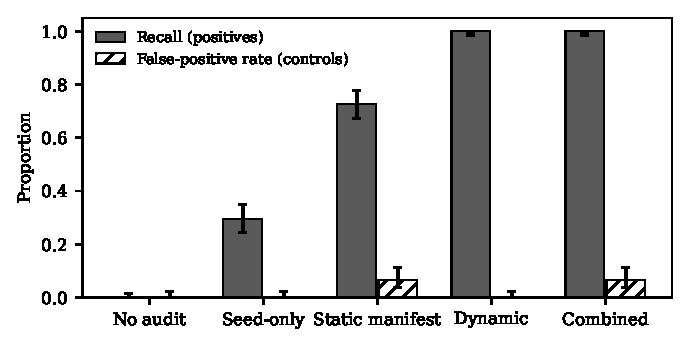
\includegraphics[width=0.78\linewidth]{figures/recall_fpr.pdf}
\caption{Recall on result-changing mutations and false-positive rate on controls, with Wilson 95\% intervals.}
\label{fig:recallfpr}
\end{figure}

The seed-only check detected exactly the 80 random-state mutations and nothing else. The static manifest detected every mutation that alters the declared configuration (198 cases) but none of the 74 hidden mutations (28 stale-cache, 28 environment-override, 18 dependency-drift). Its 12 false positives were all thread-count controls: raising \texttt{n\_jobs} for random forests and $k$-NN changes the declared configuration but not the result. The dynamic auditor detected all positives and raised no false alarms. Paired against seed-only, the dynamic auditor's recall was 70.6 percentage points higher (bootstrap 95\% CI 65.1--76.1; 192 discordant cases, all favouring dynamic; exact McNemar $p = 3.2\times10^{-58}$). Against the static manifest there were 74 discordant cases, all favouring dynamic ($p = 1.1\times10^{-22}$). All three draft hypothesis thresholds were met; we stress again that this run is exploratory.

\subsection{Blind spots by mutation family}

Figure~\ref{fig:family} breaks recall down by family. The pattern is sharp: each cheap check covers a fixed subset of families completely and the rest not at all. Caching, dependency and hidden-configuration failures were invisible to both non-executing checks.

\begin{figure}[t]
\centering
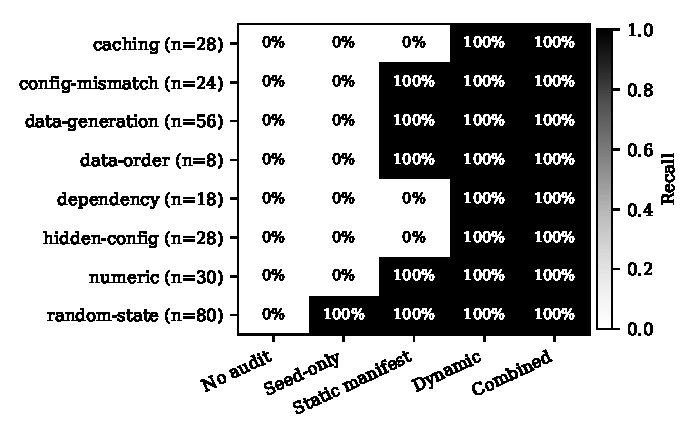
\includegraphics[width=0.78\linewidth]{figures/recall_by_family.pdf}
\caption{Recall by mutation family and method. $n$ is the number of positive cases in the family.}
\label{fig:family}
\end{figure}

\subsection{Localisation and cost}

Every method that detected a mutation also attributed it to the declared stage (seed-only 80/80, static 198/198, dynamic 272/272). For the static manifest this is partly by construction, since configuration sections map one-to-one onto stages in our design. For the dynamic auditor it is an empirical result: the first divergent fingerprint fell at the data stage in 142 cases, preprocess in 70, model in 36 and split in 24, matching the oracle in every case. Re-execution is the costliest method, with a median of 4.6 ms per audit (maximum 255 ms; 31.9 ms median for clustering experiments), roughly 50 times the static check. At this scale the absolute cost is negligible; for realistic training workloads it is not, which is why the cheaper checks matter.

\subsection{Invariances found by the oracle}
\label{sec:invariances}

The first oracle pass disagreed with 25 of 476 initially declared cases. Each disagreement was a positive that did \emph{not} change the result. We resolved them by narrowing operator applicability before the reported run, reducing the case count to 452, and record them here because they are informative in their own right:
\begin{enumerate}
  \item \textbf{Label-sorted rows with a stratified split.} Sorting the input by target before a stratified train/test split did not change any classification result (16 cases). Stratified shuffling with a stable sort selected the same rows, so data-stage artifacts differed while results did not. The operator was restricted to unstratified regression.
  \item \textbf{float32 features with tree ensembles.} Reducing feature precision to float32 left random-forest results unchanged (6 cases). The operator was restricted to non-tree models.
  \item \textbf{Loosened tolerance for a Gaussian mixture on separated clusters.} EM converged within one iteration, so loosening the tolerance changed nothing (1 case). A further 2 $k$-means cases first diverged at the metrics stage rather than the model stage; we added the clustering objective to the model-stage artifacts.
\end{enumerate}
Items 1 and 2 are natural \emph{hard controls}: intermediate artifacts change while the result does not. An auditor that compares intermediate artifacts too strictly would raise false alarms on them.

\section{Discussion}
\label{sec:discussion}

\paragraph{What the results do and do not show.} The dynamic auditor and the oracle both execute the package, so near-perfect dynamic recall on deterministic, single-fault mutations is expected and should not be read as evidence of real-world effectiveness. The informative results concern the non-executing checks: their blind spots are structural and complete. A seed check cannot see anything but seeds, and a configuration manifest cannot see anything outside the configuration. The 74 hidden mutations are exactly the cases that a careful reader of a repository's configuration would also miss.

\paragraph{False alarms have a cost.} Static comparison flagged every harmless thread-count change. In practice, false alarms train users to ignore a tool. A practical design is therefore layered: run cheap static checks always, and reserve re-execution, with at least two repeats to expose nondeterminism, for changes the static layer cannot clear or for pre-release audits.

\paragraph{Relation to studies on real repositories.} \citet{shulepov2026mutation} found that existing validation workflows in real ML repositories detected few controlled reproducibility mutations. Our controlled results suggest one mechanism consistent with that observation: checks that do not compare re-executed results against a recorded reference are blind to whole families of change. Testing this explanation on real repositories is future work.

\section{Limitations and threats to validity}
\label{sec:limitations}
\begin{itemize}
  \item \textbf{Circularity.} The dynamic auditor and the oracle share the principle of re-execution (see Section~\ref{sec:discussion}).
  \item \textbf{Synthetic, small-scale experiments.} 400-sample scikit-learn experiments on generated data; no GPU, distributed or deep-learning workloads, and no real research repositories.
  \item \textbf{Author-designed taxonomy.} The operators were chosen by the author and have not been validated against an empirical sample of real reproducibility failures; recall depends directly on which operators are included.
  \item \textbf{Simulated dependency drift} through a stand-in library rather than real package upgrades.
  \item \textbf{Single faults only}; interactions between two or more faults are untested.
  \item \textbf{One execution environment} for the benchmark run; cross-platform agreement of the benchmark itself is untested (the unit tests passed on two operating systems).
  \item \textbf{Applicability was narrowed after the first oracle pass} (Section~\ref{sec:invariances}). The narrowing was driven by the oracle, not by auditor results, but it is a researcher degree of freedom and the run is therefore not confirmatory.
  \item \textbf{Fingerprint rounding.} Hashing values rounded to 8 decimals can disagree with a tolerance comparison at rounding boundaries; no such disagreement occurred in this run.
  \item \textbf{Reproduction is not correctness.} Passing an audit does not imply that an experiment is scientifically valid.
\end{itemize}

\section{Planned work}
\label{sec:future}
Before v0.1.0 we plan to: (i) publicly preregister the hypothesis and analysis plan and run the frozen benchmark as the confirmatory study; (ii) add two-fault interactions and the hard controls of Section~\ref{sec:invariances}; (iii) run the benchmark across operating systems and library versions; and (iv) conduct a systematic literature review. Later versions will apply the operators to an independently sampled set of real research repositories under a predefined inclusion protocol.

\section{Availability}
\label{sec:availability}
Source code, experiment generators, mutation operators, auditors, oracle, tests and the raw case-level results (\texttt{results/dev-2026-11-08/cases.jsonl}, SHA-256 \texttt{a33dcec9\ldots 2828}) are available at \url{https://github.com/Hamjeth68/repromut}. Reproduce with \texttt{pip install -e ".[test]" \&\& pytest -q \&\& repromut bench --out results/full}; a full run takes under one minute on a laptop CPU. Code is released under the Apache License 2.0, documentation under CC BY 4.0 and generated fixtures under CC0.

\section*{Declarations}
\paragraph{AI assistance.} Substantial parts of the software and of this manuscript were produced with an AI assistant (Claude, Anthropic) under the author's direction. All numerical results are produced by the released scripts, and the author takes responsibility for the content.
\paragraph{Funding.} None.
\paragraph{Competing interests.} The author declares no competing interests.
\paragraph{Data.} All data are synthetic and generated by the released code; no human-subject or personal data are involved.

\bibliographystyle{plainnat}
\bibliography{references}

\end{document}
